\documentclass[10pt, landscape]{article}
\usepackage[scaled=0.92]{helvet}
\usepackage{multicol}
\usepackage{calc}
\usepackage{ifthen}
\usepackage[landscape]{geometry}
%\usepackage{hyperref}

\usepackage{newtxtext} 

%for strikeout
\usepackage{ulem}

%For editing parbox
\usepackage[table]{xcolor}
%For editing itemise margins, reduce iterm separaion and list separation
\usepackage{enumitem}
% For math
\usepackage{amsmath,amsthm,amsfonts,amssymb}

%For pictures / figures
\usepackage{color,graphicx,overpic}
\graphicspath{ {./images/} }

%\usepackage{newtxtext} 
%\usepackage{amssymb}
%\usepackage[table]{xcolor}
%\usepackage{vwcol}
%\usepackage{tikz}
%\usepackage{wrapfig}
%\usepackage{makecell}

\pdfinfo{
  /Title (CS2107-notes.pdf)
  /Creator (Ger Teck)
  /Author (Ger Teck)
  /Subject ()
  /Keywords (tex)}

%% Margins for PAPER

% This sets page margins to .5 inch if using letter paper, and to 1cm
% if using A4 paper. (This probably isn't strictly necessary.)
% If using another size paper, use default 1cm margins.
\ifthenelse{\lengthtest { \paperwidth = 11in}}
	{ \geometry{top=.3in,left=.3in,right=.3in,bottom=.3in} }
	{\ifthenelse{ \lengthtest{ \paperwidth = 297mm}}
		{\geometry{top=0.5cm,left=0.5cm,right=0.5cm,bottom=0.5cm} }
		{\geometry{top=0.5cm,left=0.5cm,right=0.5cm,bottom=0.5cm} }
	}

% Turn off header and footer
\pagestyle{empty}
% for tight centres (less spacing)
\newenvironment{tightcenter}{%
  \setlength\topsep{0.5pt}
  \setlength\parskip{0.5pt}
  \begin{center}
}{%
  \end{center}
}

% Redefine section commands to use less space
\makeatletter
\renewcommand{\section}{\@startsection{section}{1}{0mm}%
                                {-1ex plus -.5ex minus -.2ex}%
                                {0.5ex plus .2ex}%x
                                {\normalfont\large\bfseries}}
\renewcommand{\subsection}{\@startsection{subsection}{2}{0mm}%
                                {-1explus -.5ex minus -.2ex}%
                                {0.5ex plus .2ex}%
                                {\normalfont\normalsize\bfseries}}
\renewcommand{\subsubsection}{\@startsection{subsubsection}{3}{0mm}%
                                {-1ex plus -.5ex minus -.2ex}%
                                {1ex plus .2ex}%
                                {\normalfont\small\bfseries}}
% change font
%\renewcommand{\familydefault}{\sfdefault}
%\renewcommand\rmdefault{\sfdefault}
\linespread{1.05}

\makeatother

% Define BibTeX command
\def\BibTeX{{\rm B\kern-.05em{\sc i\kern-.025em b}\kern-.08em
    T\kern-.1667em\lower.7ex\hbox{E}\kern-.125emX}}

% Don't print section numbers
\setcounter{secnumdepth}{0}

\setlength{\parindent}{0pt}
\setlength{\parskip}{0pt plus 0.5ex}

%% this changes all items (enumerate and itemize, reduce margins) ITEMIZE SEPARATION HERE
\setlength{\leftmargini}{0.5cm}
\setlength{\leftmarginii}{0.5cm}
\setlist[itemize,1]{leftmargin=2mm,labelindent=1mm,labelsep=1mm, itemsep = 0mm}
\setlist[itemize,2]{leftmargin=4mm,labelindent=1mm,labelsep=1mm, itemsep = 0mm}

%itemsep = 0mm
%\setlist{nosep}

% -------------------------------------------------------------------------------

% START OF DOCUMENT HERE

\begin{document}
\raggedright
\footnotesize
\begin{multicols*}{3}

% multicol parameters
% These lengths are set only within the two main columns
%\setlength{\columnseprule}{0.25pt}
\setlength{\premulticols}{1pt}
\setlength{\postmulticols}{1pt}
\setlength{\multicolsep}{1pt}
\setlength{\columnsep}{2pt}


%% DOCUMENT NAME HERE
\begin{center}
     \Large{\textbf{CS2106 Introduction to \\
     				 Operating Systems}} \\
\end{center}
AY24/25 Sem 2, github.com/keithxun


\section{Memory Management}

\subsection{Memory Abstraction - Contigious Memory Allocation}
\begin{itemize}
\item Fixed partitioning: Internal fragmentation (small process wastes space), size need to be large enough to contain largest process
\item Dynamic partitioning: External fragmentation (many holes), need to maintain more information in OS, first fit, best fit, worst fit, buddy system (s bit of B and C is a complement)
\end{itemize}

\subsection{Paging}
\begin{itemize}
\item Logical address space divided into pages, physical memory divided into frames
\item Page table maps logical page to physical frame
\item Keep frame size as power of 2
\item Physical frame size = logicial page size
\item PA = (frame number) * (frame size) + offset
\item Internal fragmentation (last page not full)
\item Page table information stored in PCB
\item 2 Memory accesses for each logical address
\item TLB: Cache for page table, TLB hit - retrieve frame number, TLB miss - page table lookup, update TLB
\item TLB is part of hardware context switch
\item Protection: Access-bits, valid bit
\item Page sharing: Copy-on-write, shared pages
\end{itemize}

\subsection{Segmentation}
\begin{itemize}
\item Logical address space divided into segments, each segment has a name, base and limit
\item LA = <segment number, offset>
\item PA = (base from segment table) + (offset)
\item Can grow/shrink and be protected/shared independently
\item Can cause external fragmentation
\end{itemize}

\subsection{Segmentation with Paging}
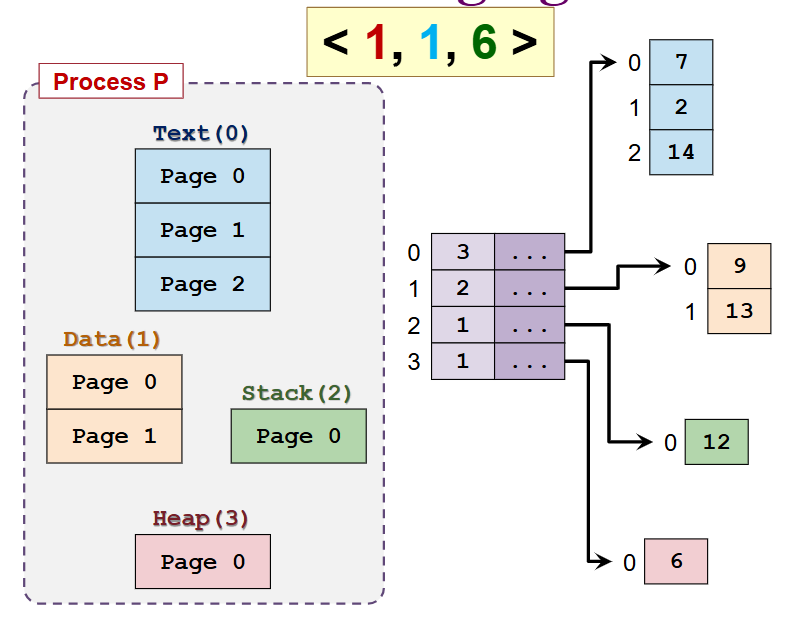
\includegraphics[width=\columnwidth]{Segmentation with Paging.png}
\begin{itemize}
\item Segment table contains page table
\item Page table contains frame number
\item LA = <segment number, page number, offset>
\item PA = (frame number from page table) + (offset)
\end{itemize}

\subsection{Virtual Memory}
\begin{itemize}
\item Secondary storage >> RAM
\item Memory resident bit in page table 
\item Page fault: page not in memory, OS handles page fault, restart
\item Temporal locality: recently used pages likely to be used again
\item Spatial locality: pages near recently used pages likely to be used
\item Demand paging: Starts with no memory resident page, only loads a page when page fault
\item Fast startup time but appear sluggish at the start
\end{itemize}

\subsection{Page Table structures}
\begin{itemize}
\item Direct paging: All entries in a single table, page table size = $2^n$ * (size of page table entry)
\item 2-level paging: 2-level page table, first level page table points to second level page table, second level page table points to frame
\item Only allocate page table entries for pages that are in memory
\item Advantage: Less memory usage, no need to allocate page table for all pages \includegraphics[width=\columnwidth]{2-level paging.png}
\item Inverted page table: Maps physical frames to $\langle$pid, page number$\rangle$, only one page table for all processes, one table for all processes but need to search for page table entry, pid + page number is unique but not page number only
\end{itemize}

\subsection{Page Replacement Algorithms}
\begin{itemize}
\item Dirty page: modified -> need to write back to disk
\item $T_{access} = (1 - p) \cdot T_{mem} + p \cdot (T_{page\_fault})$
\item FIFO: First in first out, replace oldest page, time is not updated when referenced again, more frames lead to more page faults (Belady's anomaly), does not exploit temporal locality
\item LRU: Least recently used, replace page not used for longest time, does not suffer from Belady's anomaly, need to maintain a counter/stack (able to remove entries anywhere) to track "last access time", expensive to implement, strictly increasing can lead to overflow for counter
\item Second chance: FIFO with reference bit, if reference bit is 1, give second chance, if 0, replace page
\item Optimal: Replace page not used for longest time in future
\end{itemize}

\subsection{Frame Allocation}
\begin{itemize}
\item Global replacement: All frames are shared, allow self-adjustment between processes but badly behaved process can take all frames, thrashing limited to one process but it can hog the I/O and degrade performance of other processes
\item Local replacement: Each process has fixed number of frames, no self-adjustment, can lead to underutilization of memory, thrashing process "steals" oage from other processes leading to cascading thrashing
\item Working set model: W(t, $\Delta$) = set of pages used in the last $\Delta$ time units, $\Delta$ = working set window, $t$ = time of reference
\end{itemize}

\section{File Management}
Citeria: Self-contained, persistent, efficient
\subsection{File System}
\begin{itemize}
\item Store data + metadata
\item ASCII files: Can be displayed or printed, e.g. text file, source code
\item Binary files: Have a predefined internal structure that can be processed by a specific program, e.g. executable, Java class, pdf, png, mp3
\item File operations as system calls: Create, open, close, read, write, delete, seek
\item Per-process open file table (in pcb) -> system-wide open file table -> disk
\end{itemize}

\subsection{Directory Structure}
\begin{itemize}
\item Single-level: All files in one directory, easy to implement, no hierarchy, no grouping
\item Tree-structure: Hierarchical, easy to implement, easy to navigate, easy to group
\item DAG: One copy of actual content, hard link (files only, deletion problems), symbolic link (directory or file, special link file containing path name of file, no deletion problems but larger overhead)
\item Symbolic link in unix is allowed to link to directory creating a general graph
\end{itemize}

\subsection{Disk organization}
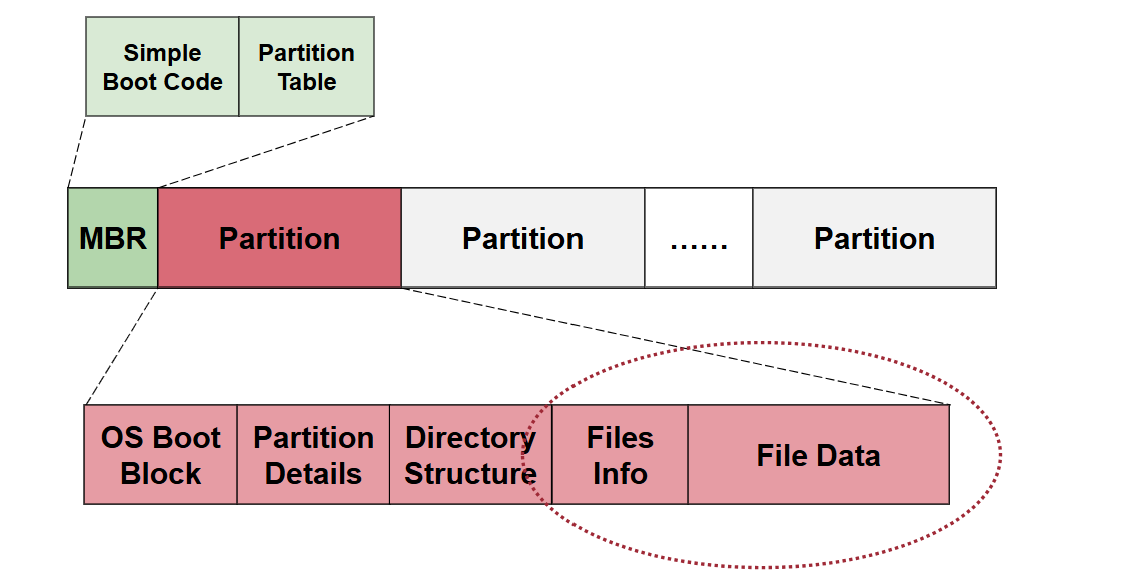
\includegraphics[width=\columnwidth]{General Disk Organization.png}
\begin{itemize}
	\item Must keep track of the logical blocks, allow efficient access, utilize disk space effectively
	\item Contiguous allocation: Simple, fast, no fragmentation, but need to know size of file in advance, external fragmentation (name, start, length)
	\item Linked allocation: No external fragmentation, but random access is very slow, part of disk block is used for pointer, less reliable (name, start, end)
	\item Linked list 2.0 (FAT): FAT is in memory at all times, simple yet efficient, FAT keeps track of the links between blocks, fast random access as traversal is done in memory but FAT can be huge and consumes valuable memory
	\item Indexed allocation: Each file has an index block (block[N] == N block address), lesser memory overhead, fast direct access but limited maximum file size and index block overhead (name, index block)
\end{itemize}

\subsection{Free Space Management}
\begin{itemize}
	\item Located in partition details section
	\item Bitmap: Each bit represents a block, 1 = free, 0 = allocated, easy to find free blocks, but slow and need to keep in memory
	\item Linked list: Each block has a pointer to the next free block, easy to locate free block and only first pointer is needed in memory but high overhead
\end{itemize}

\subsection{Implementing Directories}
\begin{itemize}
	\item Linear list: Each entry represents a file, slow linear search, solved by caching (name, start, length)
	\item Hash table: Each directory contains a hash table, fast lookup, but limited size and depends on good hash function
	\item File information: File name and other metadata, disk blocks information
\end{itemize}

\subsection{File Operations}
\begin{itemize}
	\item Create: Locate parent directory, check for duplicates, find free disk blocks, adds an entry
	\item Open: Search system-wide table for existing file entry, creates an entry in process table to point to this entry and return this pointer. If entry does not exist, locate the file and load the file information into a new entry in the system-wide table.
\end{itemize}

\section{File System Case Studies}
\subsection{Microsoft FAT File System}
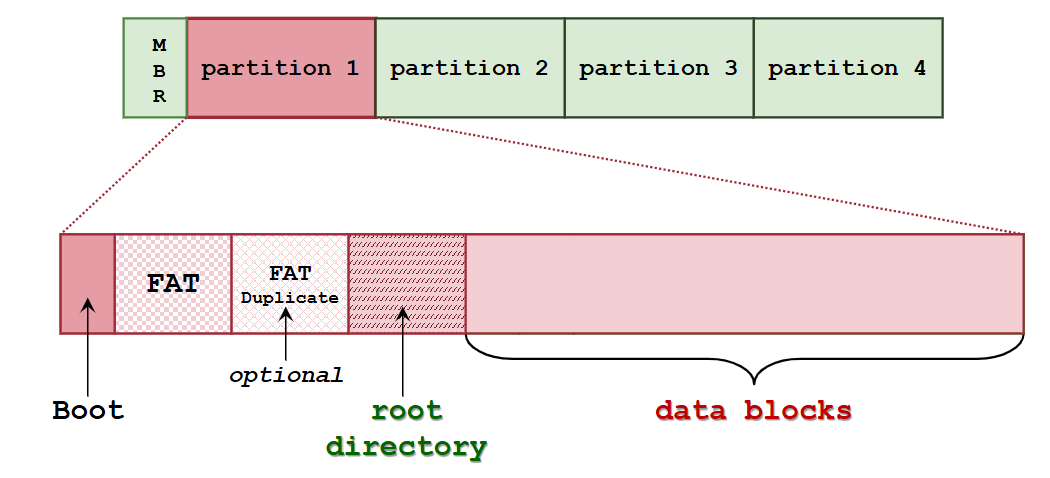
\includegraphics[width=\columnwidth]{Microsoft FAT.png}
\begin{itemize}
	\item FAT: 1 entry per data block (Free, Block number, EOF, BAD)
	\item Directory is a special type of file with root directory in a special location
	\item Directory entry in a Disk Data Block (File or subdirectory): Name + Extension (8 + 3), Creation Time and Date, First Disk Block Index
	\item First block (Directory entry) $\rightarrow$ Next (FAT) $\rightarrow$ EOF (FAT)
	\item Larger cluster size = larger usable partition but larger internal fragmentation
	\item Long file name can use multiple directory entries
\end{itemize}

\subsection{Extended-2 File System Linnux}
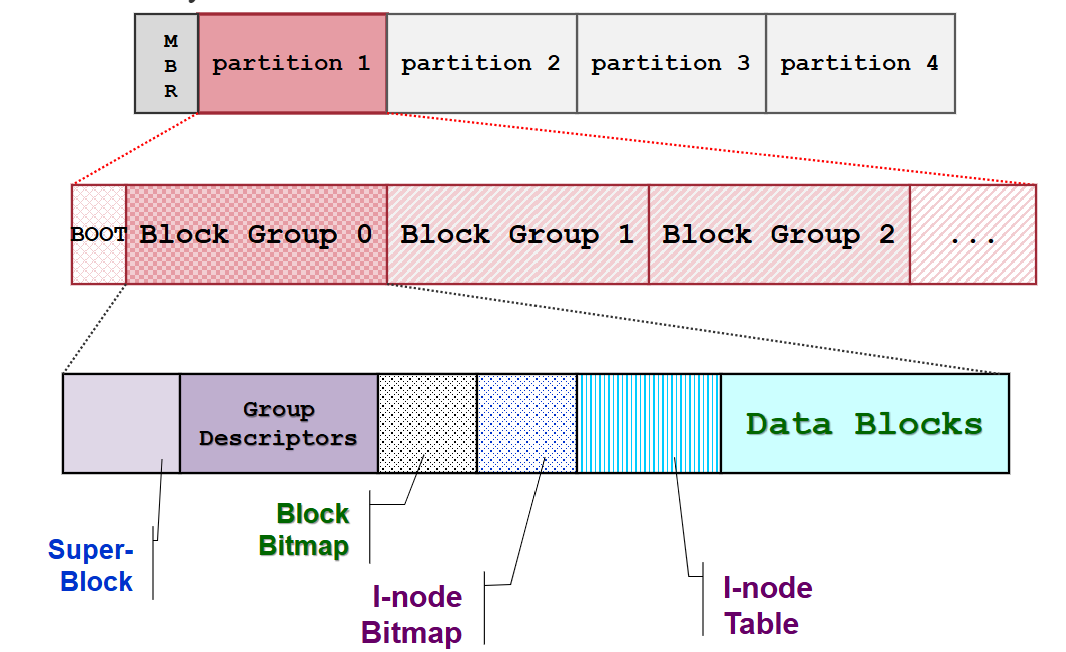
\includegraphics[width=\columnwidth]{Ext2 FS.png}
\begin{itemize}
	\item Disk space is split into blocks and then grouped into block groups
	\item Each file/directory is described by I-node which contains file metadata, data block addresses
	\item Superblocks: Describes the whole file system, total I-node number, I-node per group, Total disk blocks ...
	\item Group Descriptor: Describes the block group, number of free blocks, number of free I-nodes, location of the bitmaps, duplicated in each block group
	\item Block bitmap: Track usage status of blocks of this block group
	\item I-node bitmap: Track usage status of I-nodes of this block group
	\item I-node Table: Array of I-nodes for only this block group
	\item I-node: 15 Disk block pointers, 12 direct pointers, 1 single indirect pointer, 1 double indirect pointer, 1 triple indirect pointer
	\item Data block of directory stores linked list of directory entries within this directory
	\item Directory entry: File name, I-node number, size, length of name, type 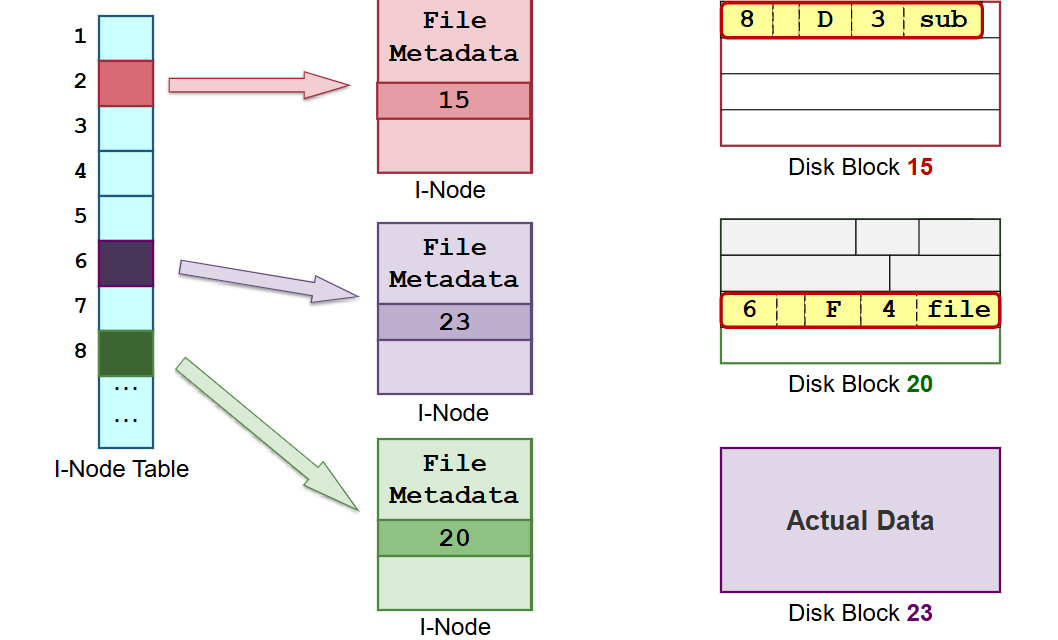
\includegraphics[width=\columnwidth]{Ext2 Inode.png}
	\item Hard link points directly to the same I-node, I-node stores reference counter
	\item Symbolic link: Special file containing the path name of the file, no reference counter
\end{itemize}

\end{multicols*}
\end{document}
